\textbf{\Large{Timeline}}

The suggested timeline for the project 
can be seen in figure \ref{timeline}, where 
the project is to start the 1. February and end 
the 31. of may. 
The first half of February will be 
spent researching related work.
A month (from mid February to mid March) 
will be spent designing and training the 
neural network. another halv a month (from mid 
March to April)
will be spent creating and testing URScripts. 
The month of April will be used to create 
the parser.
The last month, may, will be spent getting 
the final results and finishing the report.

\begin{figure}[h]
    \centering
    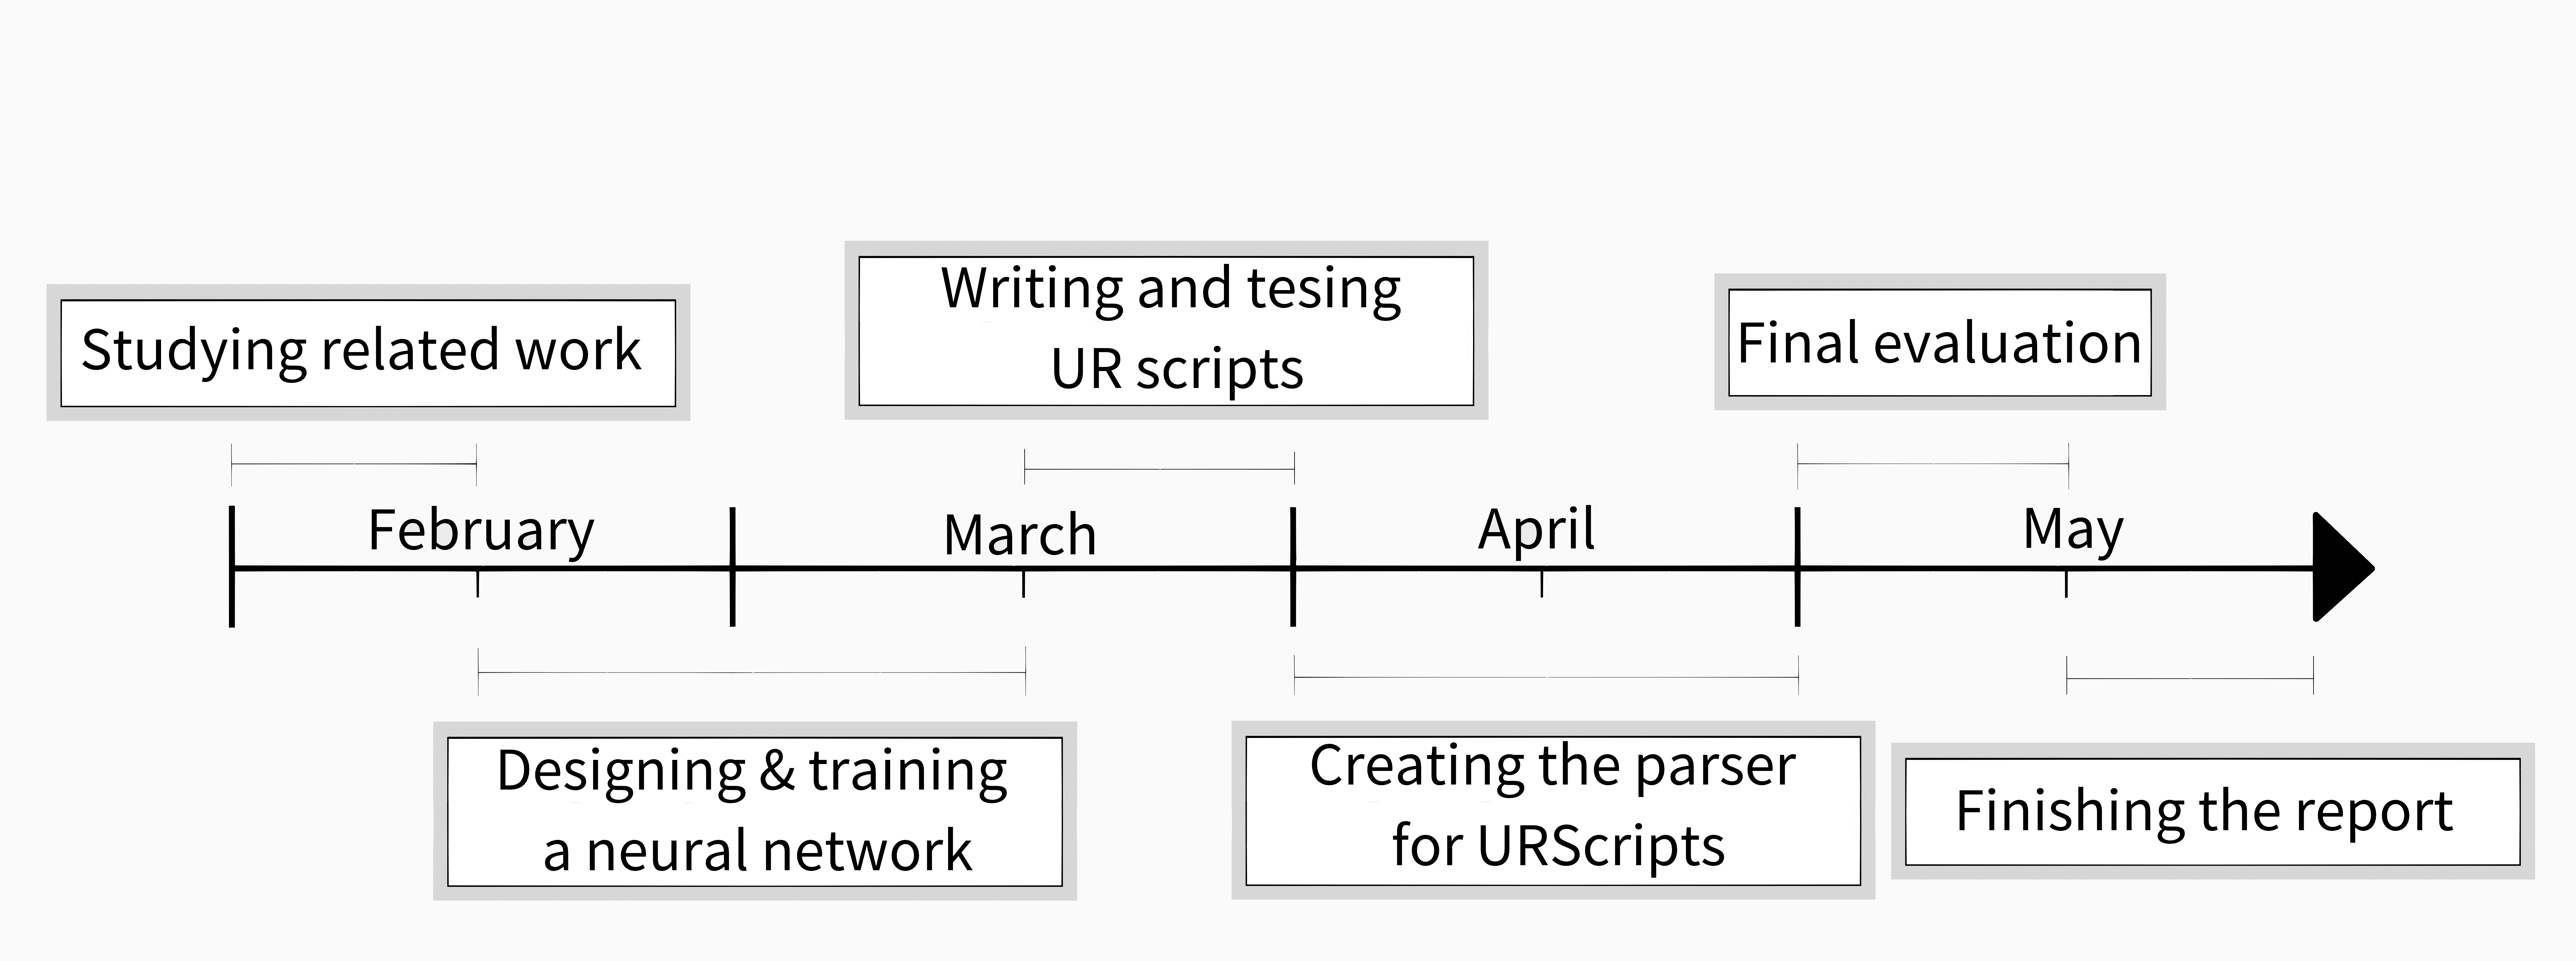
\includegraphics[width=15cm]{img/Timeline2.png}
    \caption{Suggested project timeline}
    \label{timeline}
\end{figure}


